\hypertarget{quantum-cryptography}{%
\section{Quantum Cryptography}\label{quantum-cryptography}}

\textbf{Experiment with Electrons}:\\
Elektronen sind eigentlich Teilchen und sollten sich wie solche
Verhalten. Im Experiment verhalten sich die Elektronen jedoch nicht wie
Teilchen. Werden die Elektronen jedoch beim Experiment beobachtet (ein
Observer bei Loch 1 \& 2), dann verhalten sich die Elektronen plötzlich
wie normale Teilchen. Es ist also nicht möglich, das Experiment zu
beobachten, ohne das Verhalten der Elektronen zu verändern.

\begin{figure}[H]
\centering
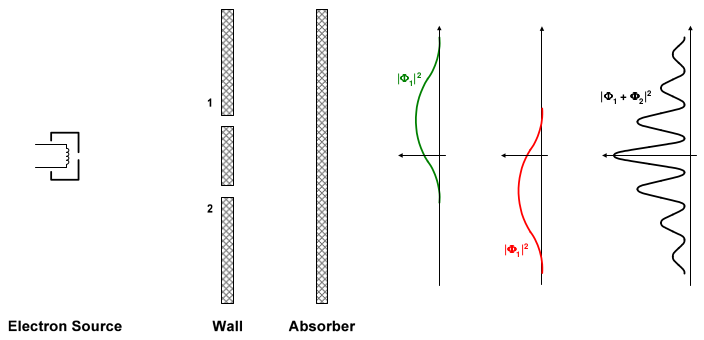
\includegraphics[width=0.8\textwidth]{figures/experimentElectron.png}
\caption{Experiment with Electrons}
\end{figure}

\hypertarget{photonen}{%
\subsection{Photonen}\label{photonen}}

Ein Photon ist die minimalste Form eines elektronischen Impulses. So ein
Photon kann man mit einem Filter polarisieren. Ein Photon das horizontal
polarisiert ist, kommt nicht durch einen vertikalen Polarisationsfilter.
Es hat jedoch eine 50\% Chance, durch einen 45° polarisationsfilter zu
kommen. Und wenn es 45° polarisiert ist, natürlich wieder eine 50\%
Chance durch einen vertikalen Filter zu kommen.

\begin{figure}[H]
\centering
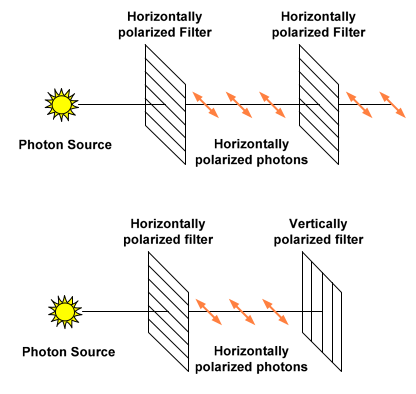
\includegraphics[width=0.5\textwidth]{figures/photonExperiment1.png}
\caption{Experiment with Photon 1}
\end{figure}

\begin{figure}[H]
\centering
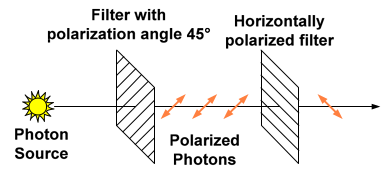
\includegraphics[width=0.5\textwidth]{figures/photonExperiment2.png}
\caption{Experiment with Photon 2}
\end{figure}

\hypertarget{definitionen}{%
\subsubsection{Definitionen}\label{definitionen}}

\textbf{Ket:} Beschreibung des Zustands vom Quantum

\textbf{Braket:} Die Wahrscheinlichkeitsamplitude in einer komplexen
Zahl. Sie zeigt die Wahrscheinlichkeit an, ob sich das Quantum von
Zustand 1 in Zustand 2 verwandelt.

\textbf{Wahrscheinlichkeit:} Die findet man, wenn man den Betrag im
Quadrat nimmt.

Beispiel dieser Definitionen im Polarisations-Experiment:

\begin{figure}[H]
\centering
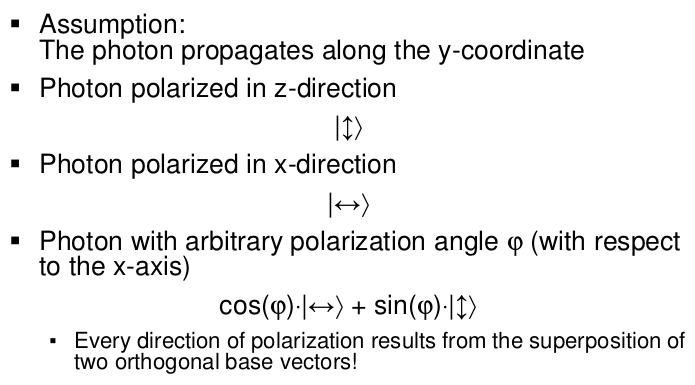
\includegraphics[width=0.5\textwidth]{figures/polarizationExample.png}
\caption{Beispiel in der Polarization von Photonen}
\end{figure}

\hypertarget{conclusion}{%
\subsubsection{Conclusion}\label{conclusion}}

Das Photon befindet sich in einer sogenannten Superposition, also im
Zustand beschrieben durch einen horizontalen Zustand UND einen
vertikalen Zustand.

\begin{itemize}
\item
  With respect to our measuring system with the basis $\{|{}\updownarrow  \rangle, |{}\leftrightarrow \rangle \}$ (vertical, horizontal) we must describe the photon polarized at an angle of 45° as:

  \begin{itemize}
  \tightlist
  \item
    \textbar{}45°$\rangle = \cos(45)*|{}\leftrightarrow\rangle + \sin(45)*|{}\updownarrow\rangle$
  \end{itemize}
\item
  The photon is in a superposition state and will make up its mind at
  the moment of the measurement whether it will pass through the filter
  or not. This decision is completely unpredictable!

  \textbf{As long as we do not make a measurement, the photon is in both
  states!}
\end{itemize}

\hypertarget{superposition}{%
\subsubsection{Superposition}\label{superposition}}

\begin{itemize}
\tightlist
\item
  Two orthogonal base vectors $|{}0\rangle$ und
  $|{}1\rangle$ $\Rightarrow$ Zwei Zustände, müssen keine Vektoren
  sein, aber Komplexe Zahlen
\item
  General form of a quantum mechanic superposition
  \begin{itemize}
  \tightlist
  \item
    $|{}\psi\rangle = a*|{}0\rangle + b*|{}1\rangle$
  \item
    a, b: complex coefficients (amplitudes)
  \end{itemize}
\item
  Measurement with respect to base $|{}0\rangle$ or $|{}1\rangle$

  \begin{itemize}
  \tightlist
  \item
    Probability for $|{}0\rangle = |a|^2$
  \item
    Probability for $|{}1\rangle = |b|^2$
  \item
    Scaling: $|a|^2 + |b|^2 = 1$
  \item
    \textbf{Das Quantum wird mit 100\% Wahrscheinlichkeit entweder 0 oder
    1 sagen.}
  \end{itemize}
\item
  The system described by $|{}\psi\rangle$ is in both states $|{}0\rangle$ und $|{}1\rangle$ at the same time
\end{itemize}

\hypertarget{entangled-states-verschruxe4nkter-zustand}{%
\subsection{Entangled States (Verschränkter
Zustand)}\label{entangled-states-verschruxe4nkter-zustand}}

\begin{itemize}
\tightlist
\item
  Several quanta can share a common state
\item
  The state of the individual quantum is not defined at the time of
  synthesis of the quanta. It will be established at the time of the
  measurement.
\item
  We have to conlcude that quantum mechanics is not local, because a
  measurement at one quantum instantaneously affects the state of
  another quantum, even if both quanta are far from each other.
\end{itemize}

\hypertarget{entanglement}{%
\subsubsection{Entanglement}\label{entanglement}}

\begin{figure}[H]
\centering
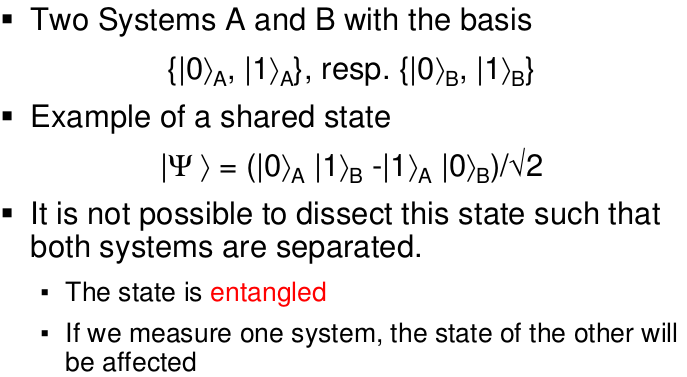
\includegraphics[width=0.5\textwidth]{figures/entanglement.png}
\caption{Entanglement}
\end{figure}

Sobald wir den einen Zustand des einen verschränkten Quantum messen und
sich der Zustand 1 herausstellt (genau in diesem Moment), ist der
Zustand des anderen Quantum in diesem Beispiel mit Sicherheit 0 (auch
wenn es Lichtjahre entfernt ist).\\
Es sind auch andere verschränkte Quanten möglich, z.B. mit 1a1b - 0a0b
$\Rightarrow$ also ist A 1, ist auch B 1.

\hypertarget{example}{%
\subsubsection{Example}\label{example}}

\begin{figure}[H]
\centering
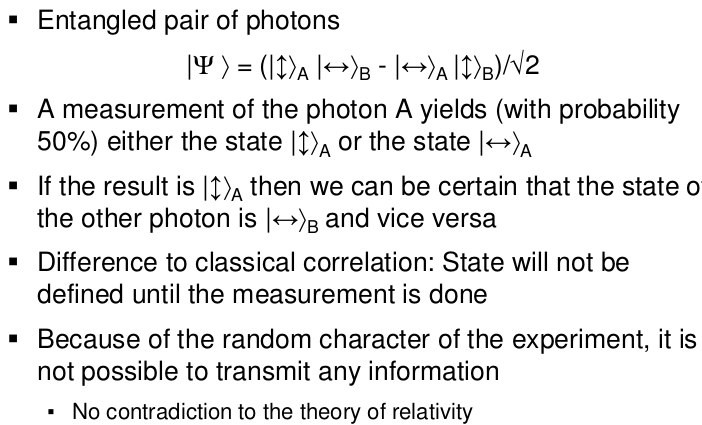
\includegraphics[width=0.5\textwidth]{figures/exampleEntanglement.png}
\caption{Example Entanglement}
\end{figure}

\hypertarget{hidden-variables}{%
\subsection{Hidden Variables}\label{hidden-variables}}

Assumption: Quanta do not decide randomly but due to some hidden
variables (that physically exist but that cannot not be measured).\\
$\Rightarrow$ Aber, die Quanten wissen nicht, was sie in Zukunft
gefragt werden. Diese Annahme kann also nicht stimmen.

\hypertarget{bells-inequality}{%
\subsection{Bell's Inequality}\label{bells-inequality}}

\begin{figure}[H]
\centering
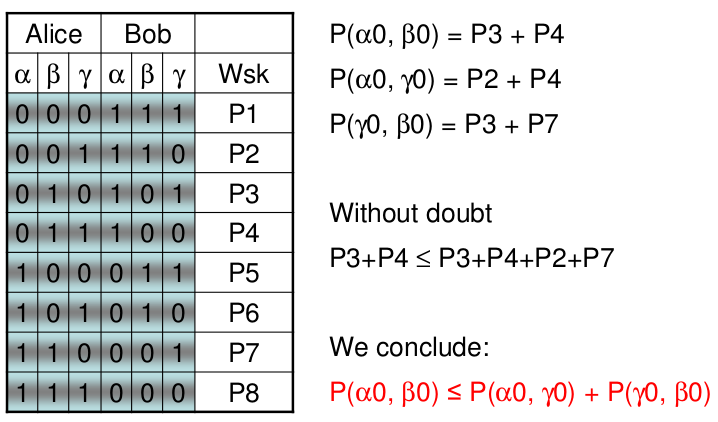
\includegraphics[width=0.5\textwidth]{figures/bellsInequality.png}
\caption{Bell's Inequality}
\end{figure}

\begin{figure}[H]
\centering
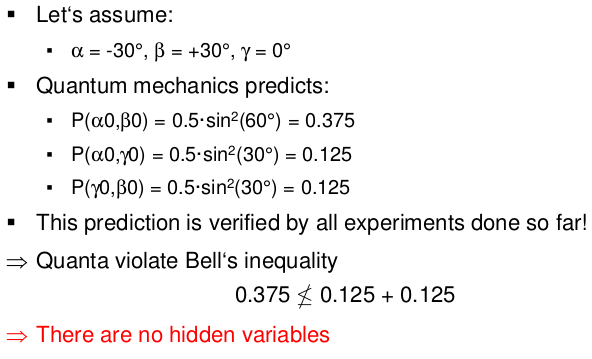
\includegraphics[width=0.5\textwidth]{figures/bellsInequality2.png}
\caption{Bell's Inequality Extended}
\end{figure}

Dieses Experiment verletzt die Voraussetzung für eine Absprache bzw.
eine Strategie. Daher wissen wir, dass es keine versteckten Parameter
gibt.

\hypertarget{no-cloning-prinzip}{%
\subsection{No-Cloning Prinzip}\label{no-cloning-prinzip}}

\emph{Für die Kryptographie wichtig.}

\begin{itemize}
\tightlist
\item
  An unknown quantum state cannot be copied.
\item
  Otherwise it would be possible to transmit information faster than
  light!
\item
  This is a fundamental difference to the classical information
  processing
\item
  Important conclusion for cryptography: An attacker may not copy quanta
  with unknown states
\end{itemize}

\hypertarget{one-time-pad}{%
\subsection{One-Time Pad}\label{one-time-pad}}

\begin{figure}[H]
\centering
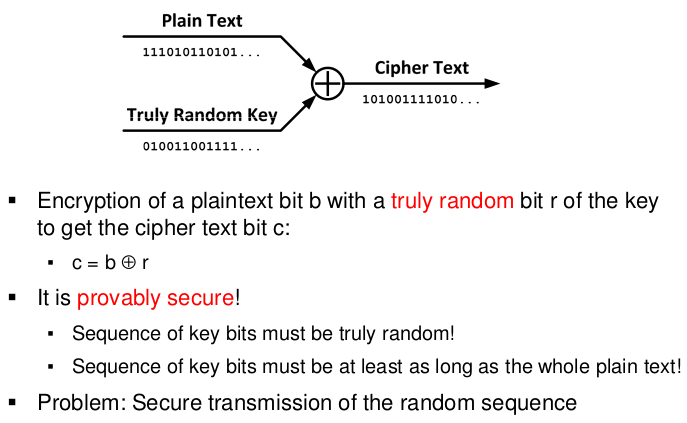
\includegraphics[width=0.5\textwidth]{figures/oneTimePadQuantum.png}
\caption{One-time-Pad}
\end{figure}

Das Problem hier ist einfach, dass man diesen zufällig gewählten sehr
langen Schlüssel irgendwie dem Empfänger über einen unsicheren Kanal
mitteilen muss.

\hypertarget{quantum-key-distribution}{%
\subsection{Quantum Key Distribution}\label{quantum-key-distribution}}

Procedure to securely exchange a shared random secret key between to
entities - The secret key can subsequently be used for a symmetric
encryption scheme such as the one time pad - It either uses quantum
superposition or quantum entanglement to implement a communication
system that allows detection of eavesdropping - Its security relies on
the foundations of quantum mechanics - No-cloning principle -
Superposition - Entanglement

\hypertarget{bb84-protocol}{%
\subsection{BB84-Protocol}\label{bb84-protocol}}

\begin{figure}[H]
\centering
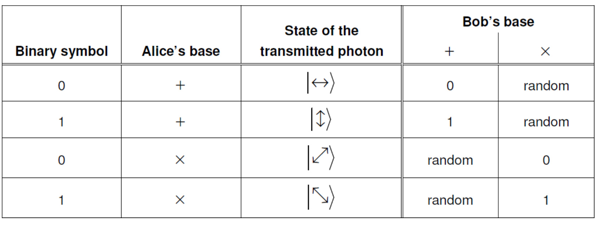
\includegraphics[width=0.5\textwidth]{figures/bb84-protocol.png}
\caption{BB84 Protocol}
\end{figure}

\begin{itemize}
\tightlist
\item
  Alice transmits polarized photons to Bob. She chooses randomly,
  whether she uses a rectilinear (+) or a diagonal (×) base
\item
  Bob measures either with a rectilinear (+) or a diagonal (×) filter.
  If he chooses the wrong filter, he will get a random result
\item
  Afterwards, Alice and Bob will exchange (over an unsecure channel) the
  information, which base they used for every transmitted photon. If
  they used the same base, the result will be a valid key bit.
\end{itemize}

\begin{figure}[H]
\centering
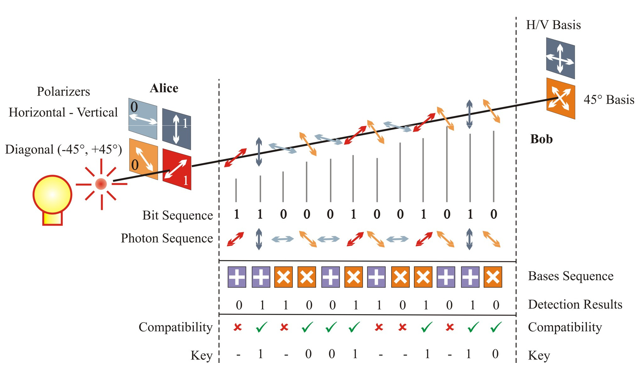
\includegraphics[width=0.5\textwidth]{figures/bb84InAction.png}
\caption{BB84 Protocol in Action}
\end{figure}

\clearpage

\hypertarget{quantum-key-distribution-with-entangled-photons-e91}{%
\subsection{Quantum Key Distribution with Entangled Photons
(E91)}\label{quantum-key-distribution-with-entangled-photons-e91}}

\begin{itemize}
\tightlist
\item
  A photon source emits a pair of entangled photons
\item
  Alice will receive photon A and randomly chooses one of the bases
  22.5°, 45° or 67.5° to perform a measurement.
\item
  Likewise, Bob receives photon B and chooses 0°, 22.5° or 45° for his
  measurement
\item
  After the transmission, Alice and Bob use an unsecure channel to
  exchange the information which base they used to measure each photon.

  \begin{itemize}
  \tightlist
  \item
    Alice and Bob used the same base. In this case, the results will be
    exactly contrary (if photon A passes Alice's filter then photon B
    will not pass Bob's filter and vice versa) and a valid symbol has
    been transmitted.
  \item
    The bases differ by 45°, yielding a completely random result. Theses
    symbols must be discarded.
  \item
    The bases differ by 22.5° or 67.5°. These measurements can be used
    to detect an eavesdropper. The probability that Alice and Bob obtain
    the same result depends on whether the photons are entangled or not.
    Any observation made by an eavesdropper will destroy the
    entanglement and thus change the probability.
  \end{itemize}
\end{itemize}

\begin{figure}[H]
\centering
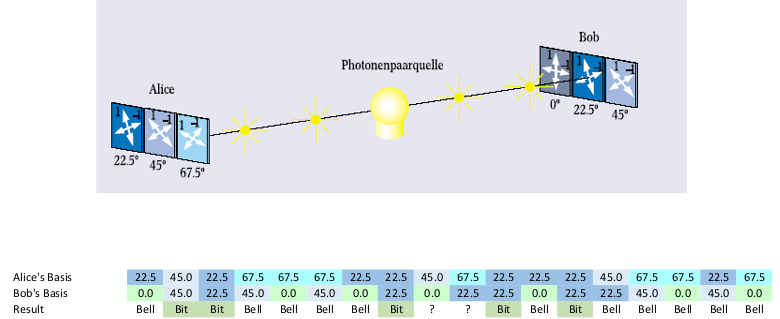
\includegraphics[width=1\textwidth]{figures/e91.png}
\caption{E91}
\end{figure}

\clearpage
